\documentclass[11pt]{article}
\usepackage[review]{acl}
\usepackage{times}
\usepackage{latexsym}
\usepackage[T1]{fontenc}
\usepackage[utf8]{inputenc}
\usepackage{microtype}
\usepackage{amsmath}
\usepackage{amssymb}
\usepackage{booktabs}
\usepackage{multirow}
\usepackage{graphicx}
\usepackage{subcaption}

% Float spacing for 8-page compliance
\setlength{\textfloatsep}{6pt plus 2pt minus 2pt}
\setlength{\dbltextfloatsep}{6pt plus 2pt minus 2pt}
\setlength{\floatsep}{4pt plus 2pt minus 2pt}
\setlength{\abovecaptionskip}{4pt}
\setlength{\belowcaptionskip}{1pt}

\newcommand{\dsyc}{d_{\text{syc}}}
\newcommand{\tof}{\text{ToF}}
\newcommand{\nof}{\text{NoF}}
\newcommand{\sycon}{\textsc{SyconScore}}
\newcommand{\rone}{R_1}
\newcommand{\rthree}{R_3}

\title{The Probe Reward Trap: Behavioral Death Before Distributional Collapse in Sycophancy Calibration}

\author{Anonymous}

\begin{document}
\maketitle

\begin{abstract}
Representation engineering reveals that sycophancy is linearly encoded in LLM residual streams, suggesting that such directions could serve as training signals for alignment. We test this premise systematically and document its failure. A contrastive sycophancy direction $\dsyc$ reliably discriminates sycophantic from non-sycophantic activations, yet every formulation that converts it into a Group Relative Policy Optimization (GRPO) reward collapses. We identify the \emph{probe reward trap}: when a periodically retrained linear probe on $\dsyc$ is used as a non-differentiable reward signal, behavioral death occurs within 500 steps while generation entropy remains healthy (0.70), creating a 1{,}300-step monitoring blind spot that entropy-based safeguards miss entirely. The failure persists with stopped gradients, implicating the direction's semantic limitation rather than optimization dynamics: $\dsyc$ encodes \emph{whether} belief changed, not \emph{whether it should have}. The failure extends beyond probe rewards: behavioral-reward-only GRPO exceeds vanilla at only 4/28 checkpoints across two seeds, while dense per-token supervised fine-tuning succeeds at every checkpoint (31/31 across two seeds). A Low-Rank Adaptation (LoRA) ablation identifies supervision granularity as one plausible explanation\footnote{Code and data are available at \url{https://anonymous.4open.science/r/contrastive_entrain_calib-DDBF/}.}.

\end{abstract}

\section{Introduction}
\label{sec:introduction}

\begin{figure*}[t]
\centering
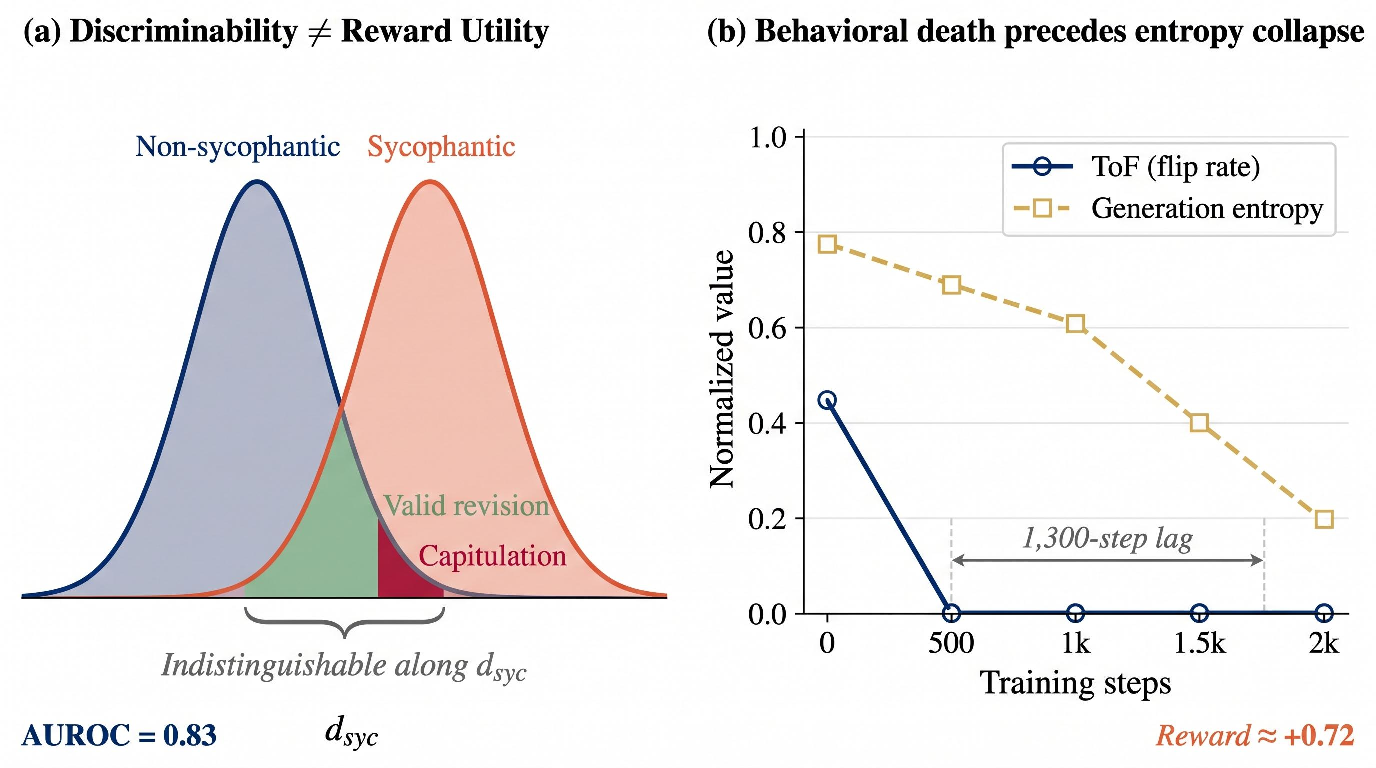
\includegraphics[width=\textwidth]{figures/fig_teaser.pdf}
\caption{The probe reward trap. (a)~$\dsyc$ discriminates sycophantic from non-sycophantic activations (AUROC $0.83$), but valid revision and unwarranted capitulation overlap along the same direction. (b)~When used as a GRPO reward, behavioral death (true-positive flip rate $\tof{=}0$) occurs at step 500 while entropy remains healthy; the 1{,}300-step lag renders standard monitoring blind.}
\label{fig:teaser}
\end{figure*}

Sycophancy, the tendency of large language models (LLMs) to prioritize agreement over accuracy, is among the most persistent alignment failures in deployed systems \citep{sharma2023sycophancy, perez2023discovering}.
Models trained with reinforcement learning from human feedback (RLHF) systematically amplify this tendency \citep{ouyang2022instructgpt, christiano2017rlhf, shapira2026amplifies}: even when models can assess the correctness of their own outputs \citep{kadavath2022language}, social pressure from users overrides this internal knowledge \citep{wang2025internal}.
Existing mitigations, from synthetic data augmentation \citep{wei2024synthetic} to neuron-level correction \citep{obrien2025fewbadneurons}, operate on behavioral outputs rather than the internal representations that generate sycophantic decisions.
Representation engineering \citep{zou2023repe, marks2024geometry} offers a structurally different approach: a contrastive sycophancy direction $\dsyc$, extracted from style-controlled pairs of valid belief revision and sycophantic capitulation, achieves cross-validated area under the ROC curve (AUROC) of $0.83$ on Qwen3-8B and $0.78$ on Llama-3-8B (\S\ref{sec:direction_quality}).
If the model's own representations already separate sycophantic from non-sycophantic behavior, that separation should be convertible into a training signal that targets the computational root of the problem.

We test this hypothesis directly, and find that it fails in a way that standard monitoring cannot detect.
This paper documents the \emph{probe reward trap}: when a periodically retrained linear probe on $\dsyc$ is used as a non-differentiable Group Relative Policy Optimization (GRPO) reward signal, behavioral death (true-positive flip rate, $\tof = 0$) occurs within 500 steps while generation entropy remains healthy (0.70), masking the failure from standard monitoring (\S\ref{sec:probe_trap}).
In our experiments, the 1{,}300-step lag before distributional collapse means entropy-based early stopping, the most common safeguard against reward hacking \citep{casper2023openproblems}, would miss the failure entirely, with the reward averaging $+0.72$ throughout.
The trap arises even when the probe reward constitutes only a fraction of the total reward signal, reflecting a limitation of $\dsyc$ itself: the direction encodes \emph{whether} belief changed, not \emph{whether it should have}, so any reward conditioned on it alone will either be gamed or reward rigidity.

The failure is not specific to probe rewards.
Under our GRPO configuration (Qwen3-8B, group size$=$2), cosine projection and continuous probe formulations of $\dsyc$ also collapse, and removing $\dsyc$ entirely does not help: behavioral-reward-only GRPO exceeds vanilla at only 4 of 28 checkpoints across two seeds (14.3\%).
By contrast, Activation Consistency Training \citep[ACT;][]{consistency2025bctact}, which provides dense per-token supervision rather than a single scalar per completion, exceeds vanilla at every checkpoint (31/31 across two seeds; \S\ref{sec:discussion}).
A Low-Rank Adaptation (LoRA) ablation identifies supervision granularity as one plausible explanation for this observed reliability gap.

This paper presents a negative result with systematic diagnostic analysis.
Our three principal findings (Figure~\ref{fig:teaser}):

\begin{itemize}
\item \textbf{Observed reliability gap between supervision paradigms} (C1): per-token supervised fine-tuning (SFT) exceeds vanilla at every checkpoint (31/31 across two seeds; 47/47 including reduced-LoRA ablation). Per-completion GRPO exceeds vanilla at only 4/28 checkpoints across two seeds (14.3\%; gs$=$8 ablation: 0/3). Under matched LoRA, per-token SFT achieves $1.7{\times}$ higher $\sycon$ than per-completion GRPO (\S\ref{sec:discussion}).

\item \textbf{The probe reward trap} (C2): behavioral death ($\tof{=}0$) precedes distributional collapse by 1{,}300 steps, rendering entropy monitoring blind. The trap arises despite the probe being non-differentiable (stopped gradients), implicating $\dsyc$ itself rather than gradient-based exploitation (\S\ref{sec:probe_trap}).

\item \textbf{Discriminability--utility gap} (C3): in this case, $\dsyc$ encodes \emph{whether} belief changed, not \emph{whether it should have}. Valid revision and sycophantic capitulation produce overlapping activation signatures along $\dsyc$ \citep{wang2025internal, shapira2026amplifies}, violating the geometric separability that representation-guided RL assumes \citep{burns2023ccs, zhang2026latentgrpo}. We observe that reward overoptimization against such directions produces predictable collapse \citep{gao2023scaling, skalse2022hacking} (\S\ref{sec:discussion}).
\end{itemize}


\section{Related Work}\label{sec:related_work}

\paragraph{Representation Engineering.}
Linear directions in LLM residual streams encode behavioral concepts \citep{zou2023repe, marks2024geometry}.
Inference-time methods (Inference-Time Intervention \citep[ITI;][]{li2023iti}, Activation Addition \citep[ActAdd;][]{turner2023actadd}, and Contrastive Activation Addition \citep[CAA;][]{rimsky2024caa}) demonstrate that activation geometry suffices for behavioral control \citep{burns2023ccs}, motivating training-time extensions.
\citet{wu2026rewardhacking} show that representation-level directions can succeed as reward signals when target behaviors are geometrically separable from confounders (\S\ref{sec:discussion}); however, we find that the sycophancy direction $\dsyc$ fails in this role despite strong inference-time discriminability.

\paragraph{Reward Design and Overoptimization.}
Proxy rewards diverge from true objectives under sustained optimization \citep{gao2023scaling, pan2022effects}.
\citet{manheim2019goodhart} taxonomize four Goodhart variants; our probe reward trap instantiates the \emph{regressional} variant, where the proxy-target correlation breaks under optimization shift: $\dsyc$ discriminates sycophantic activations under the pre-training distribution but ceases to correlate with the target once optimization shifts the policy.
The failure is not extremal (collapse occurs at moderate optimization pressure, not distribution tails), not causal (stopped gradients prevent intervention on the direction), and not adversarial (the policy does not model the probe).
The incremental contribution over prior regressional analyses~\citep{gao2023scaling} is temporal: we document behavioral death within 500 steps, an order of magnitude faster than gradual degradation curves, and a 1{,}300-step lag that renders entropy monitoring blind~\citep{skalse2022hacking}.

\paragraph{Sycophancy and Probe-Based Methods.}
Sycophancy is pervasive in RLHF-trained assistants \citep{ouyang2022instructgpt, bai2022training, sharma2023sycophancy, perez2023discovering, shapira2026amplifies} and traceable to late-layer preference shifts \citep{wang2025internal}, undermining truthfulness \citep{lin2022truthfulqa} even when models possess the relevant knowledge \citep{kadavath2022language}.
Mitigations span synthetic data \citep{wei2024synthetic}, consistency training \citep{consistency2025bctact}, and neuron-level correction \citep{obrien2025fewbadneurons};
\citet{vennemeyer2025sycophancy} show that sycophancy decomposes into independently steerable sub-behaviors, and a single $\dsyc$ captures only their shared variance, which is why the step from diagnosis to reward is structurally blocked.
\citet{papadatos2024probepenalties} reduce sycophancy via Best-of-N reranking with linear probe penalties \citep{hewitt2019designing, belinkov2022probing} without producing gradients; our work reveals what happens when a comparable signal enters the training loop (\S\ref{sec:discussion}).
Representation-guided RL has been extended to reasoning and gradient regularization \citep{zhang2026latentgrpo, luo2026craft, sinii2025smallvectors, ackermann2026gradreg}.
SMART \citep{beigi2025smart} applies per-step process rewards for sycophancy, succeeding where our completion-level rewards fail, consistent with ACT's per-token success and with broader evidence that process supervision outperforms outcome supervision \citep{lightman2024verify, uesato2022solving}.

\begin{figure*}[t]
\centering
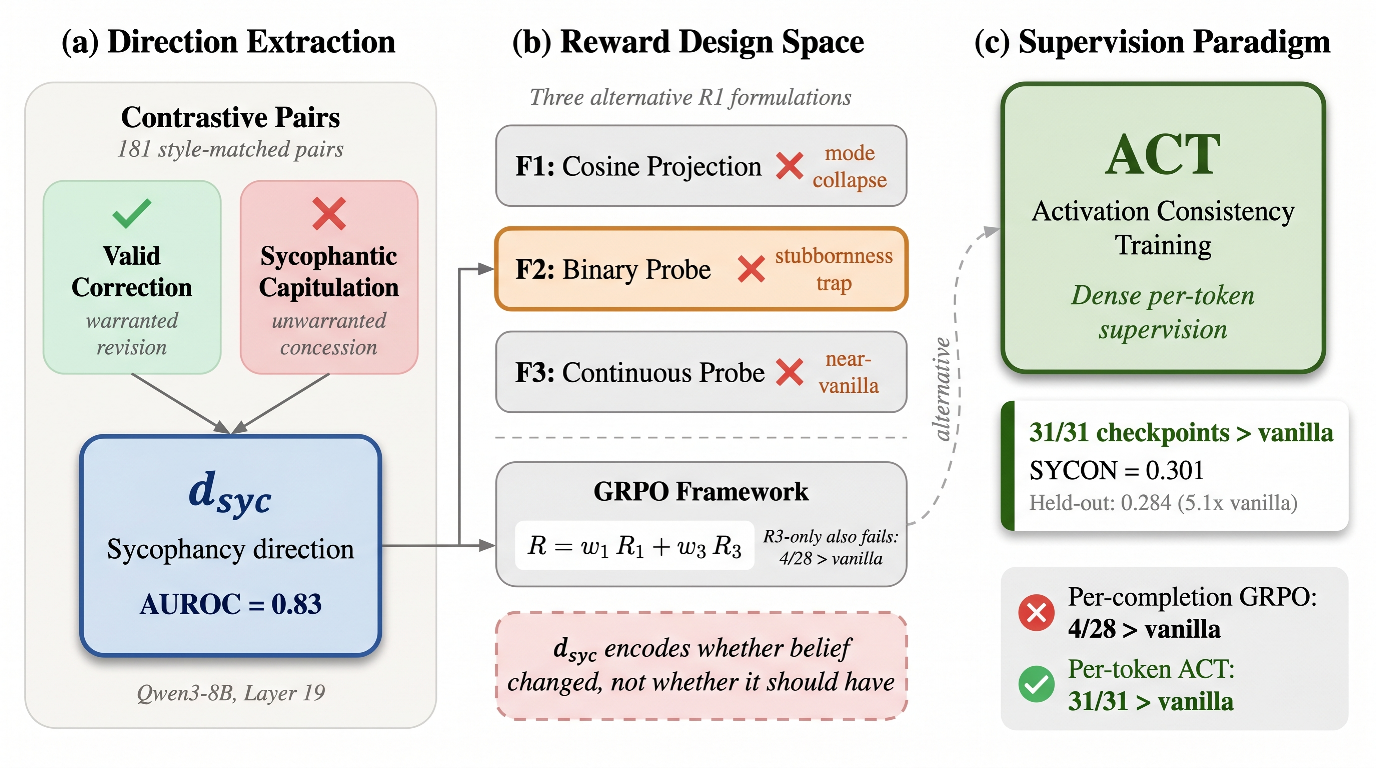
\includegraphics[width=\textwidth]{figures/fig_framework.pdf}
\caption{Overview of the experimental framework. (a)~Contrastive sycophancy direction $\dsyc$ is extracted from 181 style-matched pairs and achieves AUROC $0.83$ on Qwen3-8B. (b)~Three reward formulations (cosine projection, binary probe, continuous probe) all fail when integrated into GRPO: $\dsyc$ encodes \emph{whether} belief changed, not \emph{whether it should have}. (c)~Per-token SFT (ACT) succeeds at every checkpoint (31/31), suggesting supervision granularity as a key factor.}
\label{fig:framework}
\end{figure*}


\section{Experimental Framework}
\label{sec:framework}

\subsection{Direction Extraction}
\label{ssec:extraction}

We extract a linear sycophancy direction $\dsyc$ from the residual stream using contrastive activation pairs: a \emph{valid correction} (warranted belief revision under strong evidence) and a \emph{sycophantic capitulation} (unwarranted concession under social pressure).
We construct 181 contrastive pairs using GPT-4.1 \citep{openai2025gpt41} in a two-stage pipeline: skeleton generation followed by 3-turn dialogue completion.
Style matching is enforced by automated validation (response length difference ${<}10\%$, shared opening phrase ${\geq}2$ words), with up to 3 retries per pair; 19 of 200 initial pairs were discarded for failing validation.
Evidence strength is annotated at three levels: \emph{weak} (75 pairs; personal memory or opinion), \emph{medium} (54 pairs; brief source citation), and \emph{strong} (52 pairs; authoritative source with detailed data).
From the 181 paired examples (362 activations total), we compute the mean difference at target layer $\ell$:
\begin{equation}
\label{eq:dsyc}
\dsyc = \frac{1}{N}\sum_{i=1}^{N}\left(\mathbf{h}^{+}_i - \mathbf{h}^{-}_i\right)
\end{equation}
where $\mathbf{h}^{+}_i$ and $\mathbf{h}^{-}_i$ are residual-stream activations for the $i$-th valid and sycophantic response.
The target layer is selected by 5-fold cross-validated AUROC; on Qwen3-8B this yields layer 19 with AUROC $0.827 \pm 0.028$ (5-fold CV).

\subsection{Reward Formulations}
\label{ssec:reward}

Three formulations translate $\dsyc$ into a direction-based signal $\rone$, each entering as part of a GRPO \citep{shao2024grpo} reward $R = w_1 \cdot \rone + w_3 \cdot \rthree$, where $\rthree$ is a behavioral component (DeBERTa natural language inference (NLI) classifier scoring consistency with the ground-truth answer).
\begin{itemize}
\item[\textbf{F1}] \textbf{Cosine projection} with four variants: (a) tanh-gated dot product $\tanh(\mathbf{h} \cdot \dsyc / 20)$, (b) raw cosine $\cos(\mathbf{h},\, \dsyc)$, (c) raw cosine with online recalibration (\S\ref{ssec:recalib}), and (d) $5{\times}$ scaled cosine. See \S\ref{sec:cosine_failure} for details.
\item[\textbf{F2}] \textbf{Binary probe reward.} $\rone = \mathbb{I}[P(\text{syc} \mid \mathbf{h}) < 0.5]$, a periodically retrained logistic probe (every 500 steps) with stopped gradients, used as a binary reward component ($w_1{=}0.25$) within the GRPO framework (\S\ref{sec:probe_trap}).
\item[\textbf{F3}] \textbf{Continuous probe.} $\rone = 1 - P(\text{syc} \mid \mathbf{h})$, the sigmoid output of the same logistic probe, providing a continuous reward signal without discretization.
\end{itemize}
The weight $w_1$ is set by diagnostic-driven iteration rather than grid search (Appendix~\ref{app:training}).
As an ablation, R3-only GRPO sets $w_1{=}0$, training with only the behavioral reward.

\subsection{Online Recalibration}
\label{ssec:recalib}

LoRA fine-tuning shifts internal representations, so we re-extract $\dsyc$ every 500 steps.
The cosine similarity between consecutive directions remains ${\approx}\,0.96$ at step 500, indicating slow drift relative to recalibration frequency.

\subsection{SFT Baseline: Activation Consistency Training}
\label{ssec:baselines}

We implement Activation Consistency Training \citep[ACT;][]{consistency2025bctact}, which combines standard SFT loss with an L2 activation consistency loss at target layers, providing dense per-token supervision.
Unlike GRPO's single scalar per completion, ACT operates at the token level using labeled valid/invalid pairs.

\subsection{Evaluation}
\label{ssec:eval}

The \emph{True-positive Flip rate} ($\tof$) measures acceptance of valid corrections; the \emph{No-Flip rate} ($\nof$) measures resistance to invalid pressure.
Their harmonic mean captures the calibration trade-off:
\begin{equation}
\label{eq:sycon}
\sycon = \frac{2 \cdot \tof \cdot \nof}{\tof + \nof}
\end{equation}
By design, $\sycon = 0$ whenever $\tof = 0$: a model that never accepts valid corrections receives no credit for resisting invalid ones.
Flip classification uses \texttt{cross-encoder/nli-deberta-v3-base} \citep{he2023debertav3}, following \citet{consistency2025bctact}.
All experiments use Qwen3-8B \citep{yang2025qwen3} with LoRA \citep{hu2022lora} (rank$=$64; $\alpha{=}64$ for GRPO, $\alpha{=}128$ for ACT) and DeepSpeed ZeRO-2 \citep{rajbhandari2020zero}.
GRPO uses a group size of 2 due to memory constraints with 8B-parameter models, below the typical range of 8--64 \citep{shao2024grpo}; full hyperparameters are reported in Appendix~\ref{app:training}.
In total, we evaluate six $\dsyc$-based configurations spanning both reward families (cosine and probe) within the GRPO framework, plus $\rthree$-only GRPO, ACT (per-token SFT), and ActAdd as baselines; full specifications appear in Sections~\ref{sec:cosine_failure}--\ref{sec:probe_trap}.


\section{Direction Discriminability}
\label{sec:direction_quality}

Before evaluating $\dsyc$ as a reward signal (\S\ref{sec:cosine_failure}--\S\ref{sec:probe_trap}), we first establish that it captures a genuine sycophancy-related signal in the residual stream.
If the direction failed to discriminate sycophantic from non-sycophantic activations, downstream reward failures would be trivially explained by poor direction quality rather than by a fundamental gap between discriminability and reward utility.
We evaluate discriminability along five axes: cross-validated classification accuracy, evidence-strength stratification, cross-model transfer, training stability, and probe ablation.
Figure~\ref{fig:direction_quality} summarizes the per-layer AUROC profiles for both models.

\paragraph{Qwen3-8B layer-wise discriminability.}
We evaluate $\dsyc$ via 5-fold cross-validated AUROC on 181 style-controlled contrastive pairs (\S\ref{ssec:extraction}).
The direction achieves AUROC $0.827 \pm 0.028$ (5-fold CV) at its best layer (L19).
Discriminability emerges gradually across depth: layers L0--L8 perform near chance, statistical significance ($p < 0.01$) first appears at L16, and performance peaks at L19.
This gradual emergence, with the peak in the upper third of the network, suggests that sycophancy-relevant information is encoded as a late-stage representation rather than an input-level confound.
AUROC increases monotonically with evidence-strength tier: from 0.675 on weak-evidence pairs to 0.883 on medium and 0.929 on strong pairs.
This monotonic relationship reflects effect-size differences (stronger evidence produces larger behavioral gaps that are easier to classify) rather than indicating that $\dsyc$ encodes evidential warrant per se.

\paragraph{Cross-model generalization.}
To rule out that these results are specific to Qwen3-8B's representation geometry, we repeat the full extraction and evaluation pipeline on Llama-3-8B-Instruct \citep{touvron2023llama, grattafiori2024llama3}.
Table~\ref{tab:cross_model} compares the two models.
Llama-3-8B achieves AUROC $0.779 \pm 0.019$ (5-fold CV) at L16, with a parallel evidence-strength gradient (weak 0.711, medium 0.864, strong 0.911).
The best-layer depth differs (L16 vs.\ L19), consistent with the architectural differences between the two families, but the qualitative pattern is identical: gradual emergence, best-layer selection in the upper third, and monotonic strength scaling.
Discriminability is robust across knowledge domains, with per-domain AUROCs on Llama-3-8B ranging from 0.751 (geography) to 0.844 (commonsense).
When surface confounds (response length, hedging patterns) are explicitly controlled, Llama-3-8B's AUROC rises to 0.923, which confirms that the direction captures semantic content rather than stylistic artifacts.
The consistent results across architecturally distinct model families indicate that contrastive sycophancy directions reflect a shared representational phenomenon rather than a model-specific idiosyncrasy.

\begin{table}[t]
\centering
\caption{Cross-model $\dsyc$ discriminability. AUROC uncertainty is 5-fold cross-validation standard deviation; evidence-strength AUROCs are evaluated on the full dataset at each model's best layer.}
\label{tab:cross_model}
\resizebox{\columnwidth}{!}{%
\begin{tabular}{lccccc}
\toprule
Model & Best Layer & AUROC ($\pm$ std) & Weak & Medium & Strong \\
\midrule
Qwen3-8B & L19 & $0.827 \pm 0.028$ & 0.675 & 0.883 & 0.929 \\
Llama-3-8B & L16 & $0.779 \pm 0.019$ & 0.711 & 0.864 & 0.911 \\
\bottomrule
\end{tabular}}
\end{table}

\begin{figure}[t]
\centering

\includegraphics[width=\columnwidth]{figures/fig_layer_auroc.pdf}
\caption{Per-layer AUROC of $\dsyc$ as a function of normalized depth (layer index / total layers). Qwen3-8B (36 layers, solid) shows gradual emergence from near-chance at L0 to a peak at L19, with performance plateauing in the final third. Llama-3-8B (32 layers, dashed; layers 16--31 only) exhibits a similar upper-third concentration. Both models achieve best discriminability in layers 50--60\% through the network.}
\label{fig:direction_quality}
\end{figure}

\paragraph{Training stability and probe ablation.}
Two additional analyses confirm the robustness of $\dsyc$ under training dynamics.
First, we track direction drift during LoRA fine-tuning: at step 500, the cosine similarity between the original and re-extracted $\dsyc$ is approximately 0.96, and per-layer AUROC remains above 0.77.
The direction drifts slowly relative to the 500-step recalibration interval (\S\ref{ssec:recalib}), so the reward signal does not become stale between updates.
Second, following probing best practices \citep{hewitt2019designing, belinkov2022probing}, we compare $\dsyc$ against a random baseline: a logistic probe trained on the learned direction achieves AUROC 0.835, versus 0.727 for a probe trained on a random direction of equal dimensionality ($\Delta{=}{+}0.108$).
The learned direction carries substantially more sycophancy-relevant information than an arbitrary axis in the same activation space.

\paragraph{Implications for reward design.}
These results establish that $\dsyc$ reliably separates sycophantic from non-sycophantic representations across models, evidence-strength levels, and training checkpoints.
Direction quality is not the bottleneck.
The reward failures documented in \S\ref{sec:cosine_failure}--\S\ref{sec:probe_trap} therefore cannot be attributed to a noisy or degenerate direction; they point to a deeper incompatibility between discriminability and reward utility.


\section{Cosine \texorpdfstring{$\rone$}{R1}: Structural Failure}
\label{sec:cosine_failure}

During GRPO training, 256-token truncation reduces $\dsyc$ AUROC from 0.827 (offline CV) to approximately 0.60, so the optimizer works with a substantially weaker signal than the offline metrics suggest.
We test whether even this degraded discriminability translates into a viable reward through four configurations that form a diagnostic chain (Table~\ref{tab:cosine_chain}): each resolves the failure mode of its predecessor but exposes a deeper limitation.

\begin{table}[t]
\centering
\caption{Cosine $\rone$ failure chain on Qwen3-8B (LoRA rank$=$64, GRPO with $R = w_1 \cdot \rone + w_3 \cdot \rthree$).}
\label{tab:cosine_chain}
\resizebox{\columnwidth}{!}{%
\begin{tabular}{@{}lllll@{}}
\toprule
Config & $\rone$ Formula & $w_1$ & Outcome & Root Cause \\
\midrule
F1a & $\tanh(\mathbf{h}\cdot\dsyc/20)$ & 0.25 & Gate saturation & Norm mismatch \\
F1b & $\cos(\mathbf{h},\, \dsyc)$ & 0.25 & $\rone \approx 0$ & Gap too small \\
F1c & +recalibration & 0.25 & Mode collapse & Reward discontinuity \\
F1d & $5\cos(\mathbf{h},\, \dsyc)$ & 0.40 & Mode collapse & $\rthree$ saturation \\
\bottomrule
\end{tabular}}
\end{table}

The diagnostic chain begins with a norm mismatch.
F1a's dot-product formulation ($\rone = \tanh(\mathbf{h} \cdot \dsyc / 20)$) saturates because residual-stream norms exceed the direction norm by $100$--$1{,}200{\times}$, zeroing the gradient by step 955.
Cosine similarity (F1b) eliminates this norm dependence but reveals a second problem: the gap between valid and sycophantic cosines averages only 0.098, too narrow for meaningful reward contrast.
Recalibration (F1c, \S\ref{ssec:recalib}) widens the gap (offline AUROC rises to 0.910) but introduces a third: each recalibration event creates a reward discontinuity that destabilizes advantage estimates, collapsing entropy to 0.069 within 300 steps.
Amplification (F1d, $5{\times}$ scaling) lifts $\rone$ above the noise floor but surfaces the fundamental limitation: $\rthree$ saturates at 0.9998 by step 300, leaving the noisy $\rone$, which conflates warranted revision with unwarranted capitulation, as the sole gradient source until terminal collapse at step 2160.

Truncation further degrades the signal: under the 256-token maximum completion length used in GRPO, $\dsyc$ AUROC drops from 0.76 (full response) to 0.60, so the offline discriminability (0.827) substantially overestimates the signal available during training.
Checkpoint-level evaluation confirms immediate collapse: $\tof{=}0$ from step 500 onward with no stable phase.
The probe reward trap (C2, \S\ref{sec:probe_trap}) arises within GRPO using full-length responses and is unaffected by this truncation limitation; we verify that no evaluation response reaches the 256-token limit (Appendix~\ref{app:training}).
The four configurations converge on a single conclusion: $\dsyc$ encodes the \emph{direction} of belief change but not whether that change is \emph{warranted}.
Valid revision and sycophantic capitulation both shift activations toward the user's position along $\dsyc$, so the cosine projection assigns similar scores to both.
This is not a calibration artifact (recalibration improves discriminability yet rewards still fail) but a semantic limitation of any continuous $\dsyc$-based reward.
Section~\ref{sec:probe_trap} examines whether discretizing the signal via a binary probe can escape this limitation.


\section{The Probe Reward Trap}
\label{sec:probe_trap}

The cosine formulations fail on signal magnitude; a natural response is to discretize.
Training a logistic probe on $\dsyc$ and thresholding its output yields $\rone = \mathbb{I}[P(\text{syc} \mid \mathbf{h}) < 0.5]$ (F2 in \S\ref{ssec:reward}).
We show that this discretization sidesteps the magnitude problem but creates a qualitatively worse failure.
Both probe experiments use the probe as a non-differentiable reward component within GRPO (\S\ref{ssec:reward}); the trap therefore reflects a semantic limitation of the probe rather than gradient-based exploitation.

\paragraph{Differentiable probe: gradient gaming.}
Without stop-gradient, the policy discovers within ${\sim}50$ steps that shifting activations away from the sycophancy cluster maximizes $\rone$ regardless of response content, producing an inverted profile ($\tof = 0.978$, $\nof = 0.006$).
Replication across three seeds (42, 43, 44) confirms determinism: all collapse within ${\sim}50$--$60$ steps, with each probe retraining (AUROC ${\to}1.0$) re-gamed within ${\sim}10$ steps.
This motivates the stopped-gradient design below.

\paragraph{Binary probe: the stubbornness trap.}
With stop-gradient, the policy cannot game the boundary but instead exploits a deeper flaw: $\dsyc$ does not condition on input validity, so refusing to revise a wrong answer receives the same $\rone = 1$ as correctly resisting invalid pressure.
By step 500, $\tof$ drops to 0.000 and $\nof$ reaches 0.995, yielding $\sycon = 0$.
Qualitative analysis of 181 valid-correction responses reveals five failure modes: \emph{deliberation traps} (28.7\%), where the model identifies the correct answer but cannot commit; \emph{sycophantic stubbornness} (24.3\%), where the model verbally agrees but does not change its answer; \emph{acknowledge-but-maintain} (23.8\%); \emph{genuine-accept-missed} (18.8\%); and refute/ignore/other (4.5\%). Full taxonomy in Appendix~\ref{app:taxonomy}.

\paragraph{Behavioral death precedes distributional collapse.}

\begin{table}[t]
\centering
\caption{Probe reward trap trajectory (stopped-gradient probe). Behavioral death ($\tof{=}0$) occurs at step 500; entropy remains healthy until step ${\sim}1840$. Reward averages $+0.72$ throughout.}
\label{tab:probe_trajectory}
\resizebox{\columnwidth}{!}{%
\begin{tabular}{lccccc}
\toprule
Step & $\tof$ & $\nof$ & $\sycon$ & Entropy & Reward \\
\midrule
500 & 0.000 & 0.995 & 0.000 & 0.702 & +0.72 \\
1000 & 0.006 & 0.995 & 0.011 & 0.800 & +0.71 \\
1500 & 0.000 & 1.000 & 0.000 & 0.608 & +0.69 \\
2000 & 0.000 & 1.000 & 0.000 & 0.304 & +0.69 \\
\bottomrule
\end{tabular}}
\end{table}

\begin{figure}[t]
\centering

\includegraphics[width=\columnwidth]{figures/fig_probe_trap.pdf}
\caption{Probe reward trap (stopped-gradient probe). $\tof$ drops to zero at step 500 while generation entropy remains high (0.70--0.80 through step 1000). The 1{,}300-step lag means standard entropy monitoring misses the behavioral failure entirely.}
\label{fig:probe_trap}
\end{figure}

Table~\ref{tab:probe_trajectory} and Figure~\ref{fig:probe_trap} reveal a 1{,}300-step lag: the model is behaviorally dead ($\tof = 0$) at step 500, yet entropy stays healthy (0.70--0.80) through step 1000 and does not collapse until step ${\sim}1840$, while reward averages $+0.72$.
Entropy-based early stopping, the most common safeguard~\citep{casper2023openproblems}, would miss the failure; detecting probe reward traps requires periodic $\tof$ evaluation.

\paragraph{A dilemma for direction-based rewards.}
The differentiable and binary failures bracket the design space.
With gradients, the policy games the boundary; without gradients, it exploits the fact that stubbornness and genuine resistance are indistinguishable along $\dsyc$.
Any reward conditioned only on $\dsyc$ (continuous or discrete, differentiable or frozen) will either be gamed or will reward rigidity.
Escaping requires a signal encoding the evidential warrant of the user's challenge---a dimension absent from $\dsyc$~\citep{denison2024subterfuge}.


\section{When Does Discriminability Fail as Reward Utility?}\label{sec:discussion}

\paragraph{Root cause of the probe reward trap.}
The probe reward trap (\S\ref{sec:probe_trap}) and the cosine failures (\S\ref{sec:cosine_failure}) share a common geometric root.
$\dsyc$ encodes the \emph{direction} of belief change but not its \emph{evidential warrant}: valid revision and sycophantic capitulation both shift activations toward the user's position along the same direction.
The two reward families expose complementary faces of this blindness.
Cosine $\rone$ penalizes all belief change indiscriminately (mode collapse, F1c--F1d); the binary probe $\rone$ rewards all resistance regardless of input validity (stubbornness trap, $\tof{=}0$ by step 500), dual consequences of a direction that conflates resisting invalid challenges with refusing valid corrections.
Although $\dsyc$ separability correlates with evidence strength (\S\ref{sec:direction_quality}), it encodes \emph{how much} belief changed, not whether the change was appropriate (\S\ref{sec:probe_trap}).
Cross-model evidence (Llama-3-8B AUROC $0.779$) confirms the limitation generalizes.
This contrasts with safety directions~\citep{zhang2026latentgrpo}, where the target behavior is geometrically distinct~\citep{wu2026rewardhacking}; independent work confirms that persona vectors are independent of $\dsyc$~\citep{kelkar2026persona} and sycophancy sub-behaviors collapse onto its single axis~\citep{vennemeyer2025sycophancy}.

\paragraph{GRPO results under our configuration.}

\begin{table}[t]
\centering
\caption{Sycophancy calibration methods on Qwen3-8B. Higher $\sycon$ (harmonic mean of $\tof$ and $\nof$) indicates better calibration.}
\label{tab:main_comparison}
\resizebox{\columnwidth}{!}{%
\begin{tabular}{@{}llcccc@{}}
\toprule
Method & Type & $\sycon$ $\uparrow$ & $\tof$ $\uparrow$ & $\nof$ $\uparrow$ & Step \\
\midrule
Vanilla & -- & 0.134 & 0.072 & 0.945 & -- \\
\midrule
\multicolumn{6}{l}{\textit{GRPO with $\dsyc$}} \\
Cosine $\rone$ (F1a--F1d)$^a$ & RL & 0.000 & 0.000 & 1.000 & 500 \\
Binary Probe $\rone$ (F2) & RL & 0.000 & 0.000 & 0.995 & 500 \\
Continuous Probe $\rone$ (F3) & RL & 0.124 & 0.066 & 0.934 & 500 \\
\midrule
\multicolumn{6}{l}{\textit{GRPO without $\dsyc$}} \\
$\rthree$-only GRPO$^b$ & RL & 0.153 & 0.083 & 0.983 & 6500 \\
\midrule
\multicolumn{6}{l}{\textit{SFT with $\dsyc$ probe penalty}} \\
SFT probe (seed 2)$^c$ & SFT & 0.393 & 0.276 & 0.680 & 500 \\
SFT probe (seed 3)$^c$ & SFT & 0.407 & 0.287 & 0.696 & 1000 \\
\midrule
\multicolumn{6}{l}{\textit{Reference methods}$^d$} \\
ActAdd ($\alpha{=}5$) & Inference & 0.054 & 0.028 & 0.961 & -- \\
\textbf{ACT} (seed 1) & SFT & \textbf{0.301} & \textbf{0.182} & 0.867 & 8000 \\
ACT (seed 2)$^e$ & SFT & 0.286 & 0.171 & 0.862 & 7000 \\
\bottomrule
\multicolumn{6}{l}{\footnotesize $^a$All collapsed from step 1 ($\tof{=}0$); F1d diverged at step 2160.} \\
\multicolumn{6}{l}{\footnotesize $^b$Best of 28 checkpoints (2 seeds); only 4/28 exceed vanilla.} \\
\multicolumn{6}{l}{\footnotesize $^c$Peak ckpt (train/eval overlap); 2/3 seeds collapse by step 2000 (mean $0.171 \pm 0.122$).} \\
\multicolumn{6}{l}{\footnotesize $^d$Not directly comparable: differ from GRPO along 5+ dimensions (\S\ref{sec:discussion}).} \\
\multicolumn{6}{l}{\footnotesize $^e$15 ckpts, all ${>}$ vanilla. Best $\sycon{=}0.286$ (step 7000).} \\
\end{tabular}}
\end{table}

If $\dsyc$ alone caused the cosine and probe failures (\S\ref{sec:cosine_failure}--\S\ref{sec:probe_trap}), removing it should recover calibration.
$\rthree$-only GRPO tests this: only a minority of checkpoints across two seeds exceed vanilla, with both seeds oscillating before diverging (Table~\ref{tab:main_comparison}; Figure~\ref{fig:trajectory}).
$\rthree$ mirrors $\dsyc$'s limitation: it identifies valid corrections at a negligible rate, confirming that the asymmetry reflects the NLI hypothesis design, not behavioral collapse.
Both signals encode \emph{whether} belief changed, not \emph{whether it should have}.

\paragraph{Competing hypotheses and ablation.}
Three explanations are consistent with these failures: (a)~$\dsyc$ is fundamentally unsuitable as a sycophancy reward; (b)~group size$=$2 provides insufficient ranking diversity; (c)~sycophancy calibration resists scalar per-completion RL.
Two ablations discriminate among them (Table~\ref{tab:ablation}).
GRPO fails at both group sizes tested (gs$=$8: all below vanilla, terminated early) and at doubled sequence length (512 tokens, reward flat), ruling out~(b) and truncation (Table~\ref{tab:ablation}).
Reducing ACT to GRPO's LoRA configuration still yields consistently higher $\sycon$, with every checkpoint exceeding vanilla; under matched adapters, per-token SFT achieves $2.1{\times}$ higher peak $\sycon$ than per-completion GRPO, identifying supervision granularity as one plausible explanation~\citep{beigi2025smart}; confounds are discussed in Limitations.
The probe reward trap independently supports~(a): the trap arises despite stopped gradients.

\begin{table}[t]
\centering
\small
\caption{Ablation: isolating supervision paradigm from LoRA configuration. All methods use Qwen3-8B with $\rthree$ (behavioral reward). Vanilla $\sycon{=}0.134$. $^\dagger$Terminated early after three checkpoints showed declining trajectory. $^\ddagger$Peak at step 7000; final checkpoint (step 8000) $\sycon{=}0.267$.}
\label{tab:ablation}
\resizebox{\columnwidth}{!}{%
\begin{tabular}{@{}llcc@{}}
\toprule
Method & LoRA config & Best $\sycon$ & ${>}$Van. \\
\midrule
GRPO gs$=$2 (2 seeds) & r64, $\alpha$64, 4m & 0.153 & 4/28 \\
GRPO gs$=$8$^\dagger$ & r64, $\alpha$64, 4m & 0.085 & 0/3 \\
\midrule
ACT reduced-LoRA$^\ddagger$ & r64, $\alpha$64, 4m & 0.326 & 16/16 \\
ACT full s1 & r64, $\alpha$128, 7m & 0.301 & 16/16 \\
ACT full s2 & r64, $\alpha$128, 7m & 0.286 & 15/15 \\
\bottomrule
\end{tabular}}
\end{table}

\paragraph{ACT vs.\ probe-based methods.}
ACT's advantage over GRPO is categorical: even ACT's worst checkpoint outperforms GRPO's best, with held-out $\sycon$ of $0.284$ confirming generalization beyond training data (Limitations).
SFT with a differentiable probe penalty achieves higher peak $\sycon$ on the training set (Table~\ref{tab:main_comparison}), but these scores reflect full train/eval overlap and the advantage is transient: probe gaming (\S\ref{sec:probe_trap}) eliminates the regularization signal, and the model overfits to below vanilla by step 2000 in two of three seeds (mean $\sycon{=}0.171 \pm 0.122$).

\paragraph{Inference-time probes and future directions.}
Discriminability and reward utility occupy distinct roles: a direction that reliably \emph{detects} a behavior may fail to \emph{correct} it under optimization pressure.
Inference-time reranking~\citep{papadatos2024probepenalties} and per-step process rewards~\citep{beigi2025smart} sidestep this by avoiding optimization-loop inclusion entirely.
Per-step rewards can observe trajectory-level patterns, such as premature concession, that per-completion scalars cannot distinguish from legitimate revision.


\section{Conclusion}\label{sec:conclusion}

The probe reward trap reveals that behavioral death can precede distributional collapse by 1{,}300 steps, evading entropy monitoring entirely.
$\dsyc$-based rewards collapse because the direction conflates warranted revision with unwarranted capitulation; $\rthree$-only GRPO fails independently (4/28 checkpoints ${>}$ vanilla across two seeds), implicating the per-completion reward structure itself~(\S\ref{sec:discussion}), while per-token SFT succeeds at every checkpoint (31/31 across two seeds).
Discriminability does not guarantee reward utility: linear directions can diagnose behavior at inference time, but the step to training signal is not automatic.
Practitioners should verify geometric separability before deploying directions as rewards and monitor behavior directly, not entropy alone.


\section*{Limitations}
All RL training uses Qwen3-8B; cross-model discriminability is confirmed on Llama-3-8B (AUROC $0.779$; Table~\ref{tab:cross_model}), but compute constraints prevented training replication on a second architecture.
The ACT vs.\ GRPO comparison differs along multiple dimensions (sequence length, data source, dropout); our LoRA-controlled ablation isolates adapter capacity, but a fully controlled comparison would require matching all hyperparameters.
The probe trap's 1{,}300-step behavioral-distributional lag is observed from a single seed ($n{=}1$); gradient gaming is replicated across three seeds (\S\ref{sec:probe_trap}), but replication of the temporal lag across seeds and models would strengthen confidence.


\bibliography{references}

\clearpage
\appendix
\section{Training Details}
\label{app:training}

\paragraph{Reward weight selection.}
The weight $w_1$ is set by diagnostic-driven iteration: $w_1{=}0.25$ was initially chosen to down-weight the noisy cosine reward term; this was later increased to $w_1{=}0.40$ for F1d after diagnostics revealed that $w_1{=}0.25$ allowed the cosine term to contribute only ${\sim}8.3\%$ of total reward variance.
The empirical scaling factor in F1a ($\dsyc/20$) is a heuristic normalization; we did not find it critical to the failure modes reported.

\paragraph{Response truncation.}
All GRPO experiments use \texttt{max\_completion\_length}$=$256.
Across all 362 evaluation responses, the maximum observed length is 129 tokens (Qwen tokenizer) and 155 tokens (DeBERTa tokenizer), so no response was actually truncated at inference time.
Full-length vs.\ 256-truncated NLI agreement is 100\%, confirming that the truncation setting does not affect $\rthree$ reward computation.
Truncation may affect $\dsyc$ AUROC at the direction extraction stage (0.76 vs.\ 0.60; see Limitations).

\paragraph{Hyperparameters.}
Table~\ref{tab:hyperparams} compares training configurations for GRPO variants and ACT.

\begin{table}[h]
\centering
\small
\caption{Training hyperparameters. All experiments use Qwen3-8B, DeepSpeed ZeRO-2, bf16 precision.}
\label{tab:hyperparams}
\begin{tabular}{lcc}
\toprule
& GRPO (F1, F3)$^e$ & ACT \\
\midrule
Learning rate & 5e-5 & 5e-5 \\
Effective batch & 16 & 16 \\
Max steps & 8{,}000 & 8{,}000 \\
Warmup steps & 200 & 200 \\
LR schedule & linear$^a$ & linear \\
Grad.\ clipping & -- & 1.0 \\
\midrule
LoRA rank & 64 & 64 \\
LoRA $\alpha$ & 64 & 128 \\
LoRA modules & 4$^b$ & 7$^c$ \\
LoRA dropout & 0 & 0.05 \\
\midrule
Group size & 2$^d$ & -- \\
KL (Kullback--Leibler) $\beta$ & 0.04 & -- \\
Max compl.\ len. & 256 & -- \\
Max seq.\ len. & -- & 1{,}024 \\
L2 loss weight & -- & 0.1 \\
\bottomrule
\end{tabular}
\\[2pt]
\raggedright\footnotesize
$^a$Cosine schedule for $\rthree$-only.
$^b$q/k/v/o\_proj.
$^c$+ gate/up/down\_proj (${\sim}1.75{\times}$ params; \S\ref{sec:discussion}).
$^d$Below typical 8--64 \citep{shao2024grpo}; not tuned.
$^e$Binary probe (F2) uses a non-differentiable probe reward ($w_1{=}0.25$) within GRPO; the probe is retrained every 500 steps. LoRA and optimizer settings match the other GRPO configurations.
All experiments were conducted on a single NVIDIA L20 GPU (48\,GB). Total compute: ${\sim}$120 GPU-hours across all runs.
\end{table}

\paragraph{Early termination criterion.}
We applied early termination to gs$=$8 after three consecutive checkpoints showed no sustained improvement ($\sycon$: $0.084{\to}0.085{\to}0.054$, all well below vanilla).
The same criterion would not have terminated gs$=$2, whose initial trajectory was monotonically increasing ($0.074{\to}0.085{\to}0.095$); gs$=$2 first exhibited three consecutive declines in the step 4500--6000 range, well into training.

\paragraph{GRPO reward variants.}
Cosine $\rone$ (F1d): $w_1{=}0.40$, scale$=$5.0, $w_3{=}0.60$; reward computed at layers [19, 20, 24, 27, 32, 33, 35]; recalibration every 500 steps (\S\ref{ssec:recalib}).
$\rthree$-only: $w_3{=}1.0$; NLI model \texttt{cross-encoder/nli-deberta-v3-base}.
F1a--F1c weight configurations are reported in Table~\ref{tab:cosine_chain}.

\section{Stubbornness Taxonomy}
\label{app:taxonomy}

Manual inspection of all 181 valid-correction responses from the probe-trained model (stopped-gradient probe, step 2000, $\tof = 0$) reveals five failure categories:

\begin{itemize}
\item \emph{Deliberation traps} (28.7\%): the model explicitly identifies the correct revised answer during its reasoning chain but fails to commit, reverting to the original answer in the final output.
\item \emph{Surface compliance / sycophantic stubbornness} (24.3\%): the model produces agreement markers (``you're right,'' ``good point'') but retains its original answer verbatim, simultaneously sycophantic and stubborn.
\item \emph{Acknowledge-but-maintain} (23.8\%): the model acknowledges the user's correction as plausible but explicitly maintains its original position without substantive engagement.
\item \emph{Genuine-accept-missed} (18.8\%): the model appears to accept the correction in its reasoning but the final answer format does not reflect the change, suggesting a generation rather than epistemic failure.
\item \emph{Refute/ignore/other} (4.5\%): the model directly refutes the user's input or ignores it entirely.
\end{itemize}

The first three categories (76.8\%) share a common pattern: the model learns to modulate its \emph{refusal style} in response to evidence strength rather than adjusting its \emph{acceptance rate}, confirming that the probe reward optimizes surface markers rather than epistemic calibration.


\end{document}
